\section{Detailed Design}
	\subsection{Interface}
		\subsubsection{User Interface}
		In order to give the user intuitive control over the DRFM system a python based UI was implemented. It is a multi-threaded cross-platform interface built on the Python PyQt framework that called the Quartus TCL API \cite{PyQt} \cite{STP}. It must be noted, that all TCL interfacing was done using the adapted Altera example TCL server code\cite{TCL}.  \\ \newline The UI is made up of a menu bar, 3 sliders, and three check buttons. The menu bar allowed the user to connect to the DRFM based FPGA system or to upload data to SDRAM. The buttons enabled the user to select each of the DSP operations to be performed and the sliders give the user a fine grained control over these operations, as can be seen in Fig.~\ref{fig:UI}. 
		
		\begin{figure}[h!]
			\centering
			\begin{subfigure}{0.5\linewidth}
				\centering
				\includegraphics[width=.9\linewidth]{img/UI}
				\caption{Screen shot of the DRFM User Interface}
				\label{fig:UI}
			\end{subfigure}%
			\begin{subfigure}{0.5\linewidth}
				\centering
				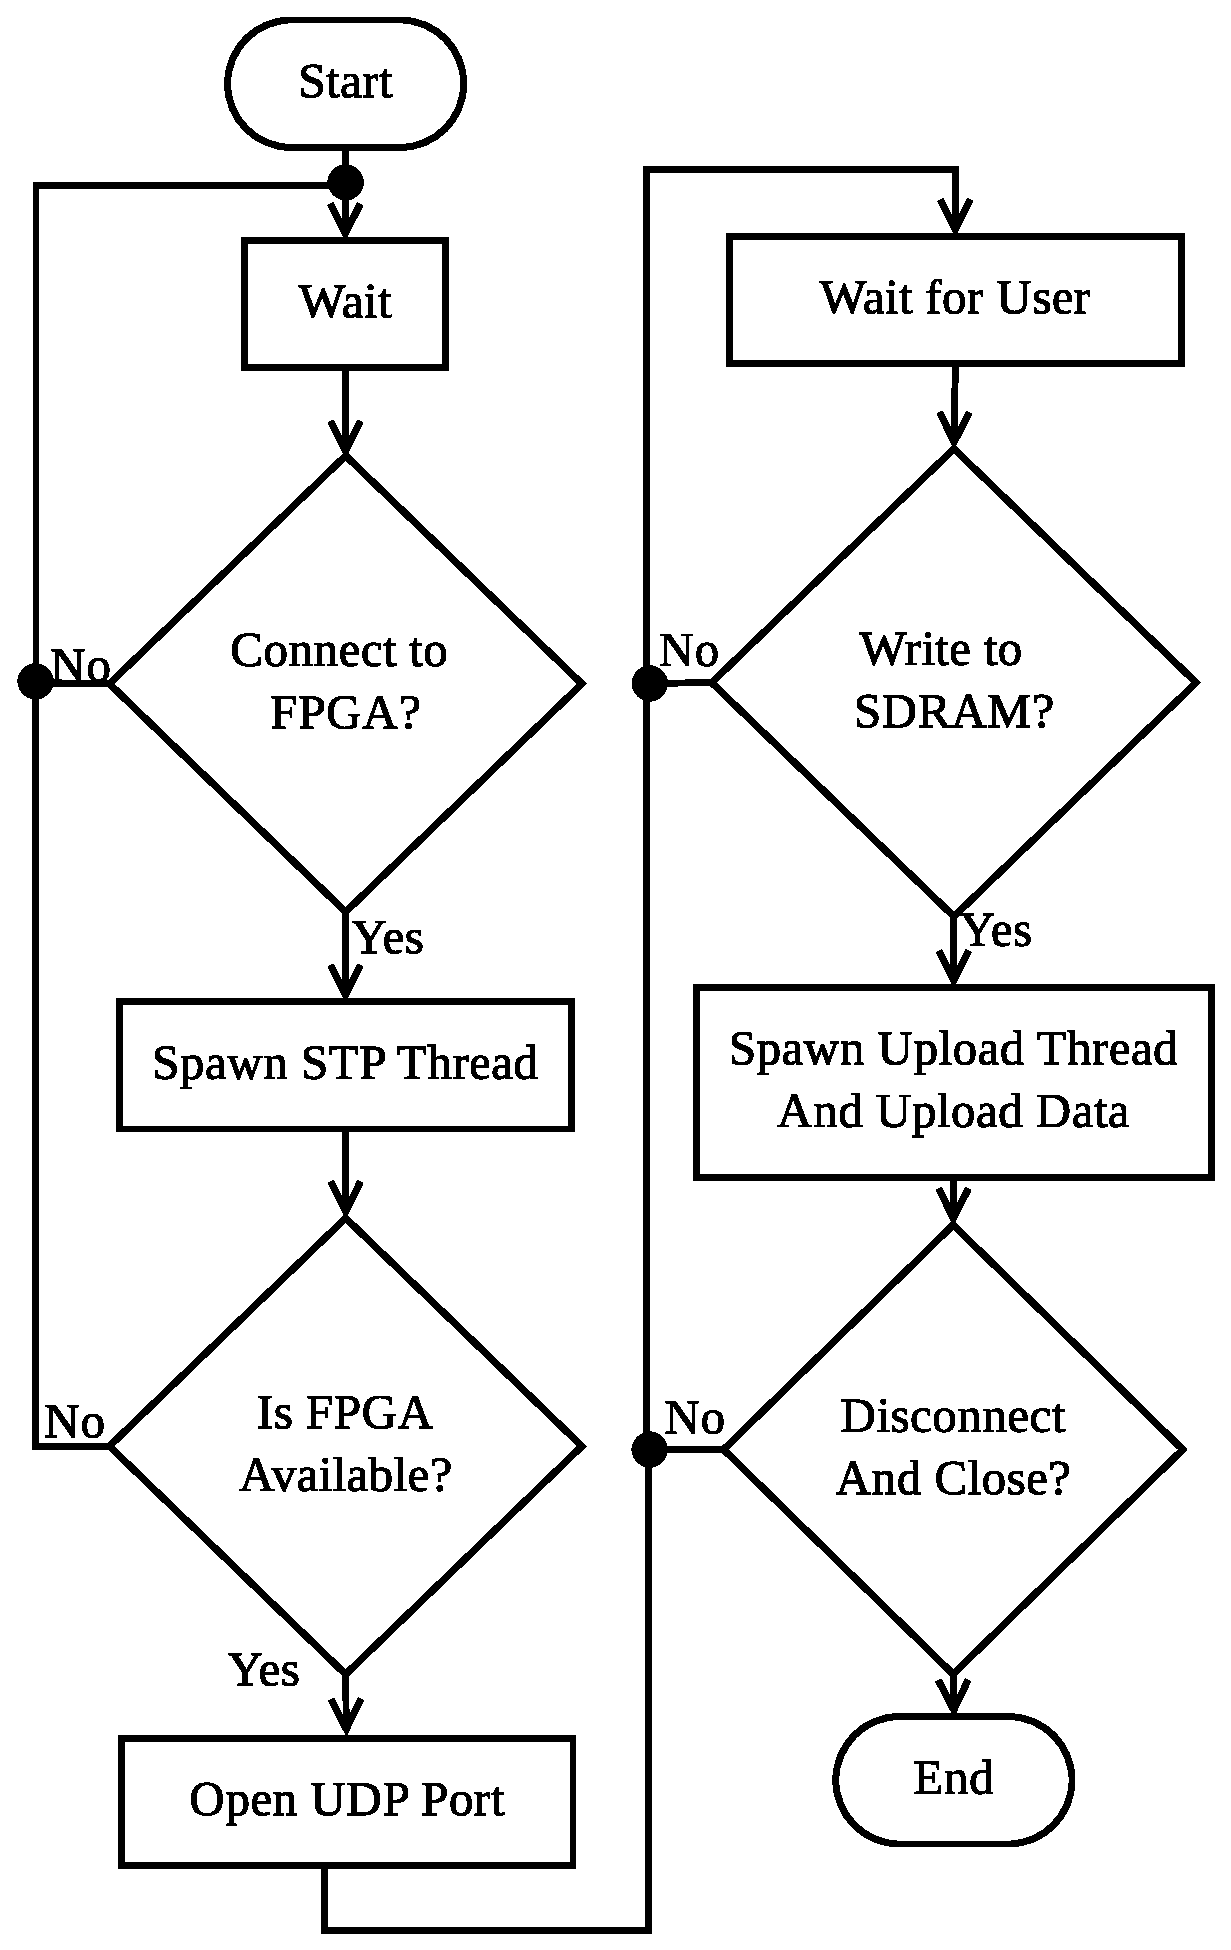
\includegraphics[width=.9\linewidth]{img/UI_Flowchart}
				\caption{Flow diagram documenting the operation of the DRFM interface}
				\label{fig:UI_flowchart}
			\end{subfigure}
			\caption{Figures documenting the DRFM interface}
			\label{fig:test}
		\end{figure}
		\noindent The way in which the interface works can be seen in Fig.~\ref{fig:UI_flowchart}. The first stage of operation is initializing the Graphical User Interface (GUI), and then waiting for the user's input. At this point, if the user connects to the FPGA a STP thread is spawned. This thread opens up a TCL server that allows for UDP traffic to be directed to the FPGA given that it is connected and available. \\ \newline From this point, the user can send control information via the check boxes and sliders through the Python socket API. At any moment after connection has been made, the user may upload data to the FPGA via the menu option and by setting switch zero (SW0) high on the FPGA development board. The data is then transferred by calling another TCL script that polls data from a pre-generated MATLAB \texttt{.dat} file and shifting the data into to the FPGA through the JTAG interface.\\
		\subsubsection{JTAG Interface}
		As previously explained, the JTAG interface was implemented using the Altera Virtual JTAG IP core for it enabled communication between the TCL server and the FPGA. The implementation thereof, required the use of the standardised JTAG interface. The pins and their descriptions can be seen in Table.~\ref{tab:JTAG_info}.
		\begin{table}[h!]
			\centering
			\caption{JTAG Interface Pin descriptions}
			\begin{tabular}{|c|c|}
				\hline
				\textbf{Pin Name} & \textbf{Description} \\ 
				\hline
				tck 	& Test Clock Input  \\
				\hline
				tdi    	& Test Data Input \\
				\hline
				tdo    	& Test Data Output\\
				\hline
				ir\_in  & Instruction Input\\
				\hline
				cdr   	& Capture Data Register\\
				\hline
				sdr  	& Shift Data Register\\	
				\hline
				udr 	& Update Data Register \\
				\hline
			\end{tabular}
			\label{tab:JTAG_info}
		\end{table}
		 \\ \newline The \texttt{tck} input is an external clock that is supplied by the TCL server that synchronizes the internal state machine operations. The \texttt{tdi} and \texttt{tdo} pins are parallel input and output data lines to and from the TCL server. The \texttt{ir\_in} output port of the Virtual JTAG IP core is the resultant output of the data that has been shifted into the instruction register of the JTAG interface. Finally \texttt{cdr}, \texttt{sdr}, and \texttt{udr} each indicate which state the finite state machine is currently in, these being, capture, shift and update states respectively\cite{JTAG}. \\ \newline These pins are then routed according to which mode of operation in DRFM system is in, either write mode or data capture mode.  \\ \newline In write mode, the \texttt{tdi} line is routed to the input of an SDRAM controller and the addressing information is incremented according to the current state the virtual JTAG controller. In data capture mode, the control information is shifted out of the \texttt{tdi} line and its contents is captured. This saved information then determines the values that are applied to the frequency shift, amplitude scaling and time delay. \\ \newline These two modes of operation are determined by the user setting SW0 on the development board. When the switch is high, the system is in write mode and when low the system is in data capture mode.   \\
		
		\subsubsection{Controller} 
		\noindent The controller module enabled the communication and routing between each of the various subsystems, for this reason it is described as part of the interface subsystem. \\ \newline  The controller receives and transmits the external peripheral data signals from the SDRAM and the PLL and routes them to and from the SDRAM Controller, JTAG interface and the DSP subsystems. In addition to this, it serves as a means to ensure the data being outputted from SDRAM is correctly handled as the SDRAM controller can not output data on every clock cycle. \\ \newline The reason for this is due to the physical properties of the SDRAM device which needs to refresh its cells regularly in order to maintain coherency of its data. During these refresh cycles, which are managed by the SDRAM controller, the SDRAM cannot ensure valid output data. Therefore during the duration of the refresh cycles the SDRAM cannot output data, and so the data output must be arbitrated, which is performed by the controller module.    \\ \newline  The arbitration employed by the controller module worked by writing the SDRAM data into a 2048 address wide RAM module. When the data was needed, it was read back from the RAM at a significantly slower speed than the writing operation was performed. This meant that when the SDRAM was unable to read data during its refresh cycles, there was sufficient data in the RAM module so that its output appeared unchanged.\\ \newline Furthermore, data was only written from the SDRAM to the RAM block when the \texttt{Read\_DataValid} line from the SDRAM was high and was only read from the SDRAM to the RAM block when the   \texttt{Read\_WaitRequest} was low.  \\ \newline Finally, the controller module also performed the changes in assignment for when the SDRAM was being written to or read from. The way this was done was by having duplicates of the inputs to the SDRAM controller, and reassigning them when the switch on the FPGA development board was toggled.
		
	
	\subsection{Peripheral Interfacing}
		\subsubsection{SDRAM Subsystem}
		As already mentioned, the Altera SDRAM Controller IP Core \cite{SDRAM_Core} was implemented  through the use of Altera's Qsys integration tool. This was done so to abstract the internal details of the SDRAM system. A functional block diagram of the SDRAM Controller core can be seen in Fig.~\ref{fig:SDRAM_core}.
		
		\begin{figure}[h!]
			\centering
			\includegraphics[width=0.95\linewidth]{img/SDRAM}
			\caption{Block Diagram Demonstrating Interfacing SDRAM \cite{SDRAM_Core}}
			\label{fig:SDRAM_core}
		\end{figure}
		\noindent The Avalon-MM interface is the part of the SDRAM controller that is visible to the higher level controller block. It abstracted the external SDRAM ports to a simpler interface that enabled its integration into the DRFM system. \\ \newline  Practically, the interface abstracted most of the lines so that only  the data, data valid, wait request, write address, read address and read/write lines had to be considered when reading and writing from SDRAM. This meant that the top level controller module was able to drive Avalon-MM Slave interface as described above. \\ \newline This was because the Avalon-MM slave port supports external SDRAM peripheral controlled wait states for when the external SDRAM device is not capable of receiving or sending data. This is as a result of the external SDRAM peripheral periodically refreshing its cells. This means, that in order to overcome these problems, the slave port interface employed the use of wait request and read data valid lines. So that when the external SDRAM peripheral was in its refresh state, the top level controller module could wait until it was capable of receiving data again. \\
			\subsubsection{PLL}
		As shown in Fig.~\ref{fig:SDRAM_core}, the implementation of the DRFM system required for the fundamental clock frequency to be altered in order to effectively communicate with the external SDRAM chip. In order, to do this the Altera Phase Locked Loop (PLL) IP Core was incorporated into the design\cite{PLL}. \\ \newline A PLL is a closed loop frequency control system that works by comparing phase difference between the reference input clock signal and the feedback clock signal from the voltage controlled oscillator. This information about the error in phase of the two signals is then used to control the frequency of the loop. The main components of a PLL can be seen in Fig.~\ref{fig:PLL}. 
		
		\begin{figure}[h!]
			\centering
			\includegraphics[width=0.95\linewidth]{img/pll}
			\caption{Block Diagram of the Internal Structure of the PLL IP Core \cite{PLL}}
			\label{fig:PLL}
		\end{figure}
		\noindent The fundamental elements of the Altera PLL are the Phase Frequency Detector (PFD), Charge Pump, Loop Filter, Voltage Controlled Oscillator (VCO), and Counters and Dividers, such as a Feedback Counter (M), a Pre-Scale Divider (N), and Post Dividers (K and V). \\ \newline A feature of the Altera PLL IP Core was that it offers a locked output signal that goes high when the output is in phase with the input. Therefore, in order to ensure the system was synchronous with the PLL the bitwise inverse of locked line was used as a reset port of each module. Such that when the PLL was not locked to the input signal's phase, the system would not output and all output lines would be pulled to ground. \\ 
		
%		\subsubsection{External SDRAM}
		\subsubsection{PWM Module}
		The Pulse Width Modulation (PWM) module was used as a debugging mechanism in the DRFM system to verify that the frequency shifter module was changing the frequency correctly. The PWM output was probed with an oscilloscope with FFT capabilities so that the output frequency could be measured accurately. \\ \newline As the system clock was 100MHz and the PWM output had an 8-bit resolution the maximum bandwidth that could be outputted through the PWM module was $100\times10^6 / (10)(2^8) \approx 40kHz$. This is because the PWM frequency is required to have at least 10 times the signal's bandwidth.\\ \newline Furthermore, due to fact that the output from the DSP subsystem was 32-bits wide meant that the output had to be concatenated down from 32 bits to 8 bits. However, this resolution was sufficient for system testing and verification, but lead to various harmonics being present within the output wave form. Nonetheless, the fundamental frequency component was still clearly present in the probed output. 	


	
	\subsection{Digital Signal Processing Subsystems}
		\subsubsection{Delay}
		As already explained, the delay module was implemented through the use of a dual port RAM block. Practically, the time delay was achieved by injecting a portion of the input signal into RAM and indexing previous values of the input signal. In the implementation of the DRFM system, a dual port, 1024 address long, 16 bit wide RAM was implemented internally on the FPGA.\\ \newline The limitations of this were that 1024 samples had to be maintained in the RAM, thereby inhibiting the DRFM system from being able to output data for first 1024 clock cycles of operation. Naturally, this is an overhead of any DRFM system as real-time data must be sampled and stored. However, once the capacity criteria of the RAM had been met a single sample may be outputted every clock cycle. \\ \newline For this reason, the signal processing chain was structured as it is. This was because had a user defined variable frequency shift occurred before the delay, the RAM would have had to be refilled as previous values of the frequency shifted signal would need to be outputted.  \\ \newline  Finally, the system also took into account that when the user changed the delay input, the subtraction from the current address should only occur once. For example, if the current address pointer of the delay RAM was 1024 and the user changed the delay to 256, then the RAM address should change to 768 and the address pointer should address sequentially from that point. This means that the previous delay input was kept track of, so that only when the new user input delay was different to the old delay would the RAM change its address. \\
		\subsubsection{Arbiter}
		As the SDRAM was only 16 bits wide and each I/Q sample was 16 bits wide, the I/Q data had to be interlaced into the RAM when being injected. This meant that as the frequency shifting operations required both I/Q samples simultaneously the data had to be arbitrated to perform the addition and multiplication operations of Equation.~\ref{eq:shift}.  \\ \newline This process was achieved through the use of a simple finite state machine that had 2 states, the read I data state and the read Q data state. In the read I state the first address from RAM was stored in the arbiter as a temporary variable. In the read Q state, the subsequent address was outputted from the arbiter to the frequency shifter and a ready flag was pulled high. This finite state machine may be seen in Fig.~\ref{fig:arbiterfsm}.  \\ \newline 
		
		\begin{figure}[h!]
			\centering
			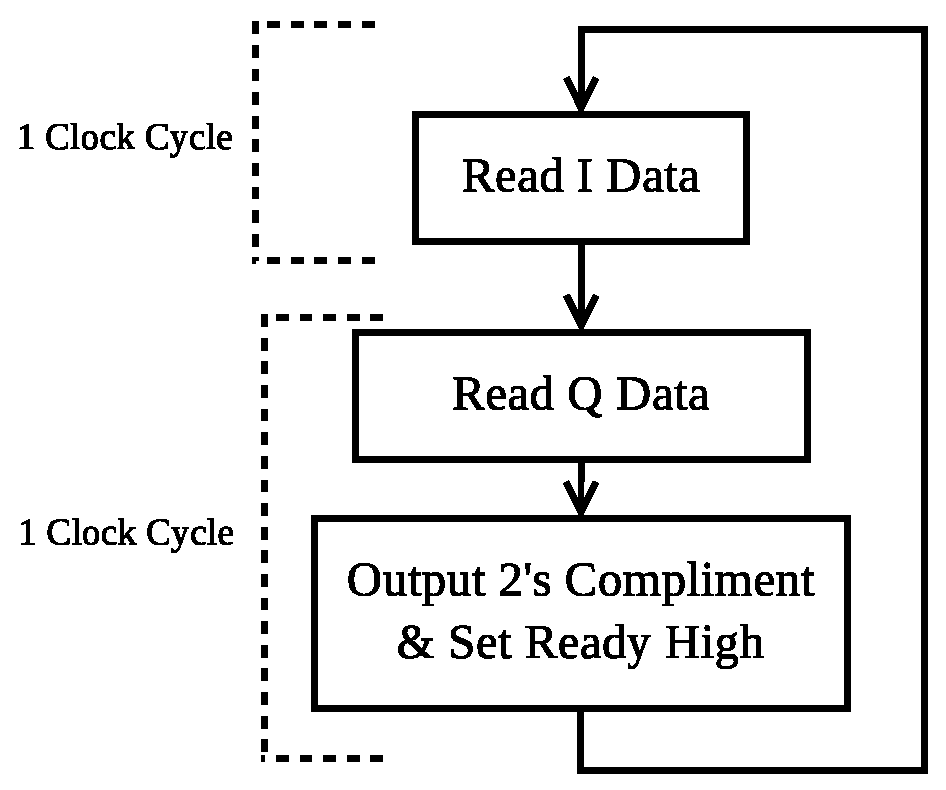
\includegraphics[width=0.52	\linewidth]{img/Arbiter_State_Machine}
			\caption{Flow chart of the Arbiter Finite State Machine }
			\label{fig:arbiterfsm}
		\end{figure}
	
		\noindent In addition to this, the arbiter module outputted a full scale 2's compliment version of the inputted I/Q data injected to SDRAM. The way in which this is done was by inverting the first bit of the I/Q Data word and appending it to the rest of the word. So in the case of the 16 bit data word, the 15th bit was inverted and bits 14 down to 0 remained unchanged. \\		  
		\subsubsection{Frequency Shifter}
		The frequency shifter module used in this DRFM system followed the exact mathematical model described by Equation.~\ref{eq:shift}. As per the derivation, the implementation required four multipliers, an addition and a subtraction, in order to result in the frequency shifted I/Q data. For this reason, the frequency shifter subsystem can be described in two parts. These being the Numerically Controlled Oscillator (NCO) and the arithmetic units. \\ \newline The NCO is an oscillator that uses a look up table, an adder and a memory to output periodic waveforms as shown in Fig.~\ref{fig:NCO}. In this case, the periodic waveforms are sin and cos, as they are required to map the complex exponential frequency shift to a realisable model. The way the NCO worked was by receiving an input frequency word that was integrated to obtain a phase that could be addressed on a Look Up Table (LUT). The LUT was implemented through the use of a 4096 address long 16-bit wide dual port ROM that was pre-initialized with a MATLAB generated Memory Initialization File (MIF). The MIF file's contents was a 100Hz sinusoid that was sampled at $2^{12}$Hz. 
			
		\begin{figure}[h!]
			\centering
			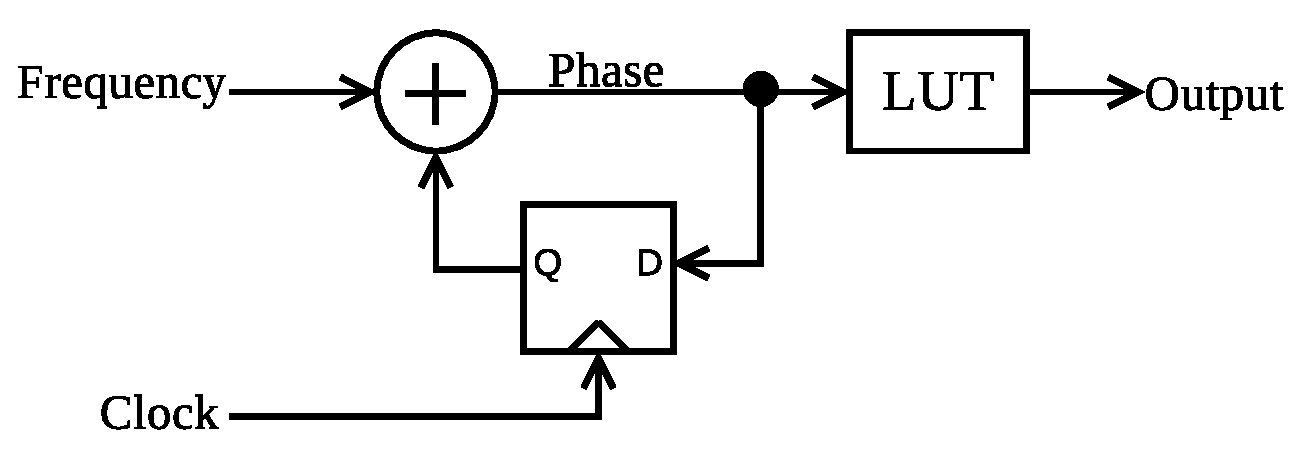
\includegraphics[width=0.7\linewidth]{img/NCO}
			\caption{Functional Block Diagram of an NCO}
			\label{fig:NCO}
		\end{figure}
		
		\noindent Furthermore, in order to generate both the cosine and sine signals that were needed for the frequency shift, two $90^\circ$ out of phase pointers were used. Digitally, the $90^\circ$ phase shift translated into the pointers being 1024 addresses apart. \\ \newline Finally, in order to scale the user inputted frequency shift into a frequency shift a translation had to be performed. This translation can be expressed mathematically as 
		\begin{equation}
			f_{shift } = f_{slider} \dfrac{2^{32}}{100MHz}
		\end{equation}
		\noindent where $f_{shift}$ is the instantaneous frequency that the NCO must output, $f_{slider}$ is the user input in kHz, $2^{32}$ is the frequency word resolution and 100MHz is the clock frequency. \\ \newline The second part of the frequency shifter was the arithmetic subsystem. A block diagram of the arithmetic subsystem may be seen in Fig.~\ref{fig:freq_shift}. It can be seen that the arithmetic operations mirror exactly what is described in Equation.~\ref{eq:shift}. The intricacies of these arithmetic operations lie within the binary representations of the outputs of each arithmetic operation. As the input data is 2's complement the system had to keep track of the signed-ness of each of the results. These being that the multiplication operation had to check that the 32 bit result overflowed correctly, thereby maintaining the resultants sign.  \\ \newline This was achieved by outputting the result to a 33 bit temporary vector and checking its Most Significant Bit (MSB). If the MSB was high it meant that the output was negative, then it checked if the subsequent bit was high, if it was, it meant that the result had not overflowed and the bits 31 down to zero were outputted. However when the subsequent bit was low, meant that the result had overflowed and \texttt{0x8000 0000} was outputted as it was the biggest negative 32 bit number. Conversely, if the MSB bit was low, implied that the result was positive, which meant that the subsequent bit had to be inspected. If it was high, it meant that result had overflowed and \texttt{0x7FFF FFFF} was outputted as it was the largest positive 32 bit number in 2's compliment notation. However if the subsequent bit was low meant that the result had not overflowed and that bits 31 down to zero could be outputted.
		
		\begin{figure}[h!]
			\centering
			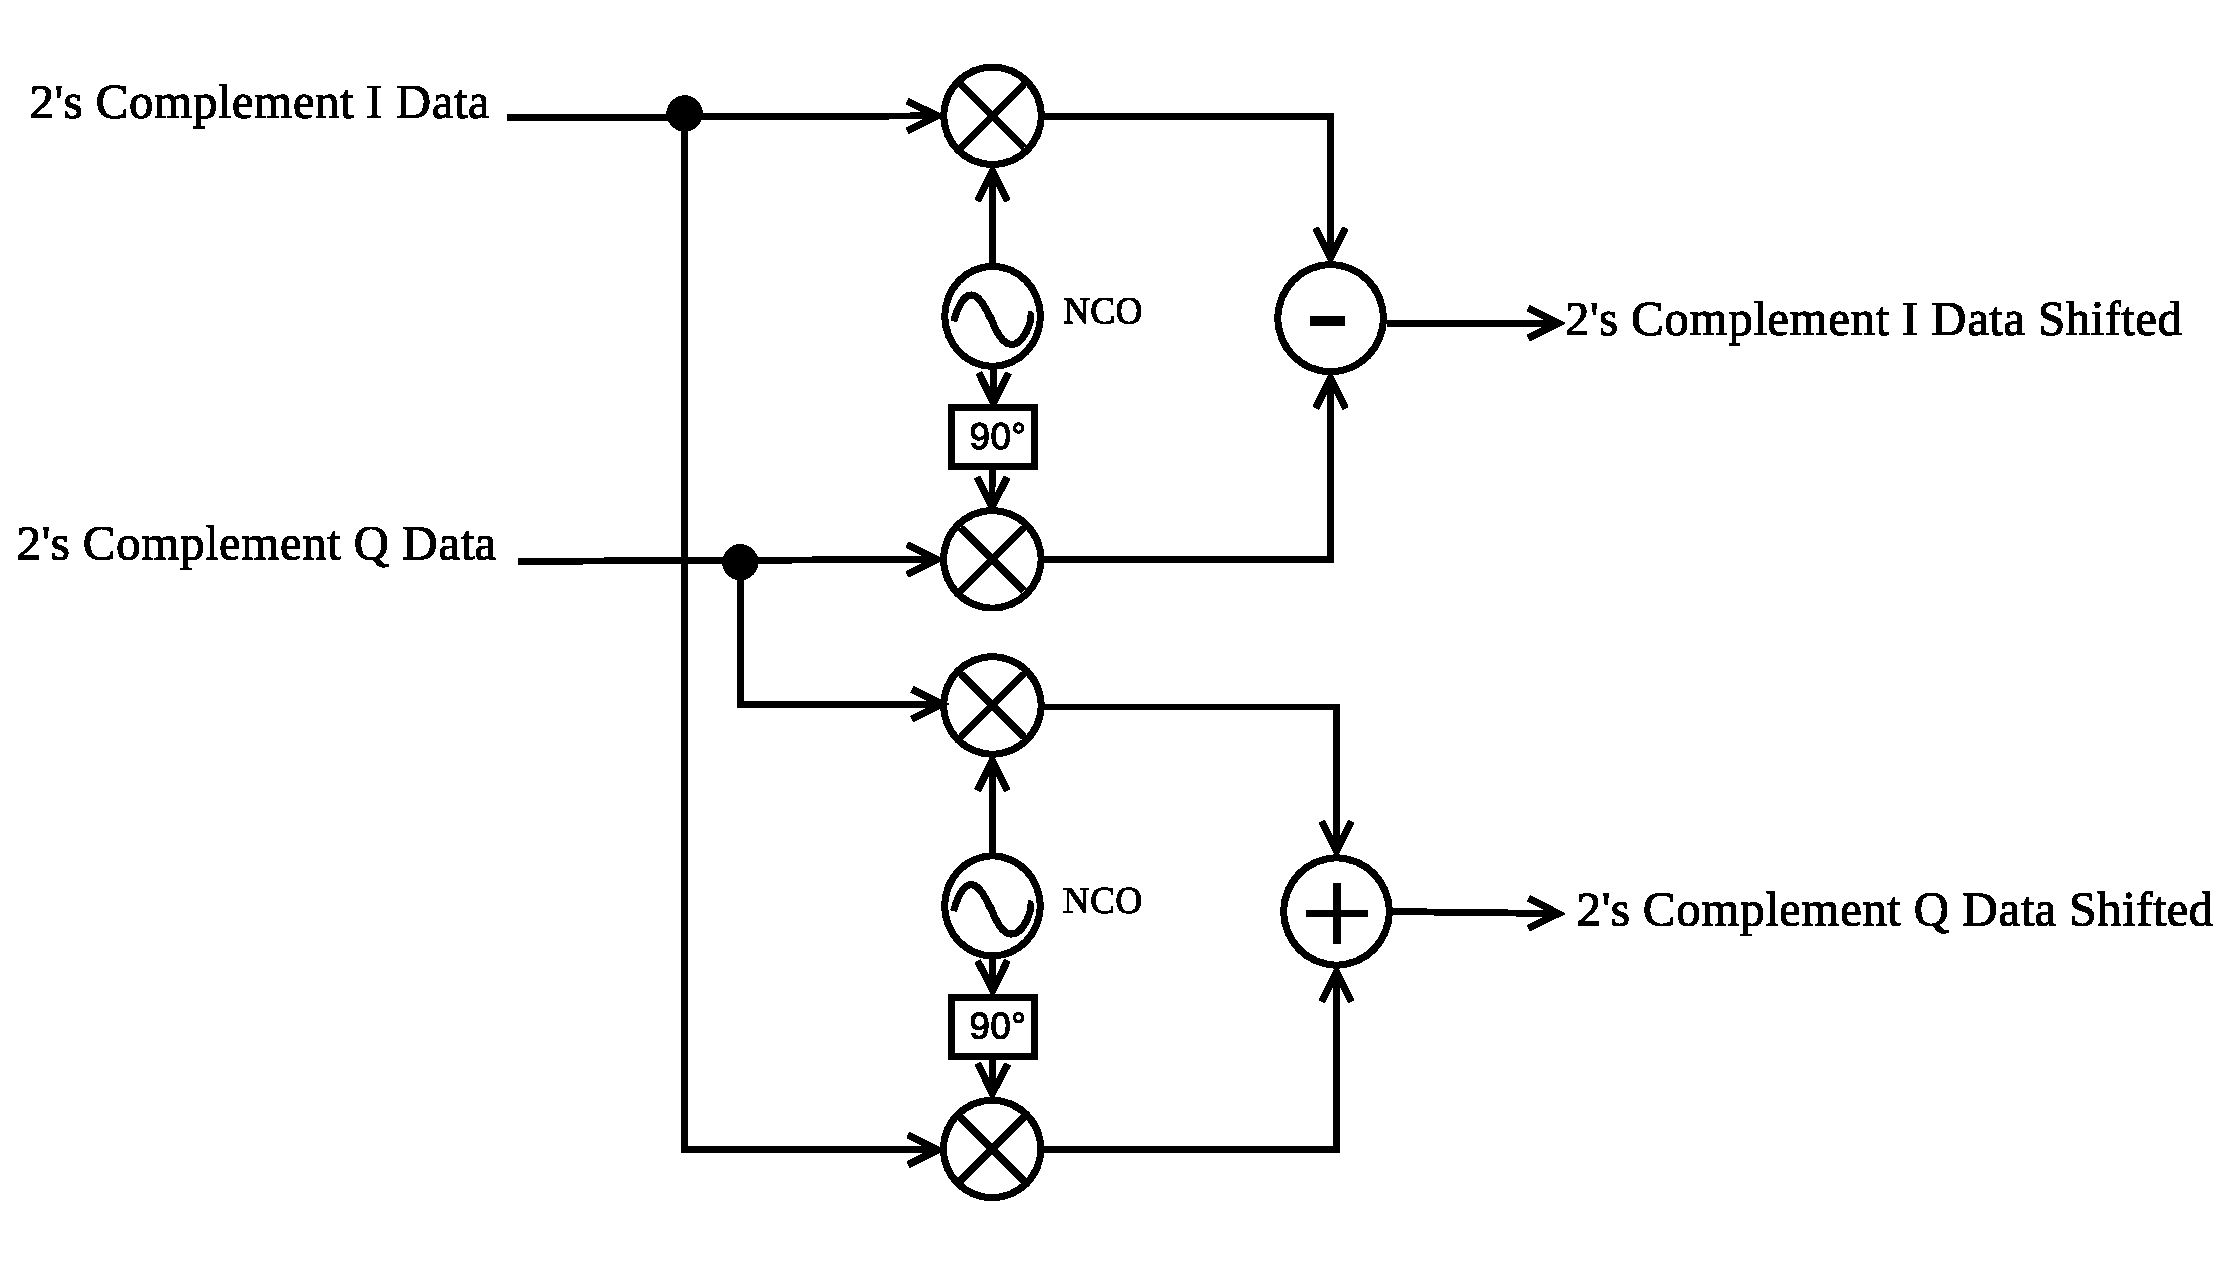
\includegraphics[width=0.8\linewidth]{img/Freq_Shift}
			\caption{Diagram of the Arithmetic Elements of the Frequency Shifter}
			\label{fig:freq_shift}
		\end{figure}
		
		\noindent Naturally as all the arithmetic operations performed in the frequency shifter chain were 2's complement, the same method of ensuring that no overflows had occurred were done in the multipliers, the subtracter and the adder. \\ \newline Finally, the only difference between the addition and subtraction operations was that the subtraction operation applied a 2's complement inversion of the Q Data before performing the addition. This is a result of the properties of 2's complement notation, in that if you do a bitwise inverse of a 2's complement number and then add 1, the result is a negated version of the original bit stream.\\
	
		\subsubsection{Scaler}
		As already explained the scaler module worked by applying a bit shifted multiplication on the incoming I/Q data and the amplitude scaling control word. This was implemented by applying a non circular shift to the amplitude scaling control word by 32 bits to the right and the I/Q data by 16 bits to the left. So that the resultant vectors were 48 bits wide. This was done to translate the scaling operation into a multiplication of the I/Q data with the amplitude scaling control word that had been translated between one and close to zero. \\ \newline Finally, the I/Q data that was received by the amplitude scaling module was the unsigned, delayed and frequency shifted version of the original data. This meant that an unsigned multiplication had to be done, such that the negative and positive overflows never had to be considered.
